\chapter{Performing a Simulation}
\graphicspath{ {./Lab00HowTo/howTo20 Performing Simulation/Fig} }

If you are planning on performing a simulation of your design then the
top level entity should be a testbench. Inside the testbench should be
an instantiation of your design as the unit under test.

\begin{enumerate}
\def\labelenumi{\arabic{enumi}.}
\item
  Click on the Files tab in the \emph{Project Navigator} pane.
\item
  Right click on \emph{topLevelProjectFile.v} in the \emph{Project
  Navigator} pane and select Set as Top-Level entity.
\item
  Click on the Hierarchy tab in the \emph{Project Navigator} pane.
\item
  In the main Quartus II window, click on \emph{Processing
  -\textgreater{} Start -\textgreater{} Start Analysis \& Elaboration.}
  This may take some time, so be patient.
\item
  You can close the compilation report by clicking on the x in the red
  box,
\item
  You should see \emph{topLevelProjectFile.v} as the root entity in the
  Hierarchy tab in the \emph{Project Navigator} pane.
\item
  In the main Quartus II window, click \emph{Tools -\textgreater{} Run
  Simulation Tool -\textgreater{} RTL Simulation}. The ModelSim program
  will launch. This may take a few moments, be patient.
\item
  In ModelSim, find the \emph{Library} pane. Expand the \emph{work}
  library by clicking on the ``+'' at left. Right click on
  \emph{topLevelProjectFile} and click \emph{Simulate}.
\item
  In the sim pane, right mouse click on uut and select \emph{Add Wave}.

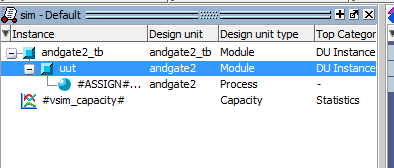
\includegraphics[width=0.4\paperwidth]{image1.png}

\item
  Choose \emph{Simulate -\textgreater{} Run -\textgreater{} Run 100}.
  You should see inputs and output from \emph{topLevelProjectFile}.
\item
  If you are asked to save the waveform. Perform the following steps:

  \begin{enumerate}
  \def\labelenumii{\alph{enumii}.}
  \item
    Undock the Wave pane by clicking the undocking tool icon.



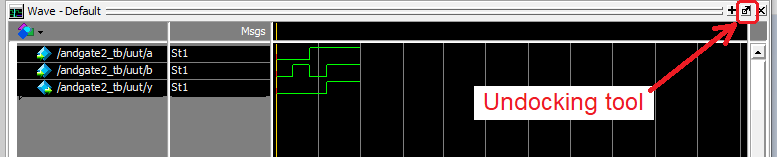
\includegraphics{image2.png}


\item
  Resize the undocked Wave window vertically by grabbing its top edge
  and dragging down. Make the window tall enough to fit all the waves
  with a little room to spare.

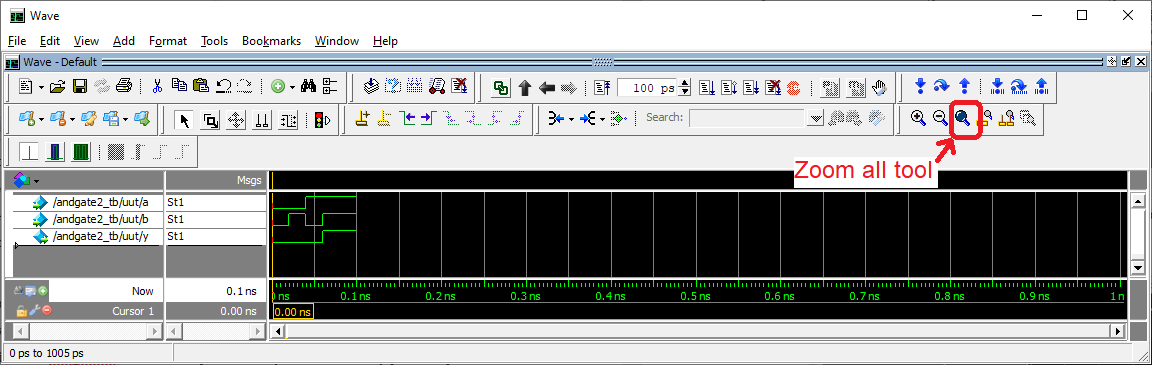
\includegraphics{image3.png}

\item
  Click the Zoom all tool to file the available horizontal space with
  the waveform.
\item
  Re-order the waves so that the inputs are highest and outputs are
  lowest. Do this by grabbing their name and dragging it to the correct
  location.
\item
  Color the intermediate signals (p1, p2, p4, p7) yellow by right
  clicking on them, selecting properties. In the View tab of the Wave
  Properties pop-up, click the Colors\ldots{} button for Wave Color and
  choose Yellow, click Close, then OK.
\item
  Color the output signals red. Leave the input signals green.
\item
  Click File -\textgreater{} Export -\textgreater{} Image
\item
  Navigate to your project directory, provide a File name, then click
  Save
\end{enumerate}

\item
  Close ModelSim. Do not save wave commands.
\end{enumerate}

